\documentclass[10pt]{article}
\usepackage[polish]{babel}
\usepackage[utf8]{inputenc}
\usepackage[T1]{fontenc}
\usepackage{amsmath}
\usepackage{amsfonts}
\usepackage{amssymb}
\usepackage[version=4]{mhchem}
\usepackage{stmaryrd}
\usepackage{graphicx}
\usepackage[export]{adjustbox}
\graphicspath{ {./images/} }

\title{LIGA MATEMATYCZNA \\
 LISTOPAD 2010 \\
 SZKOŁA PONADGIMNAZJALNA }

\author{}
\date{}


\begin{document}
\maketitle
\section*{ZADANIE 1.}
Rozwiąż równanie \(x^{2}+y^{2}=x+y+2 \mathrm{w}\) zbiorze liczb całkowitych.

\section*{ZADANIE 2.}
Wypisujemy kolejno liczby według następującej reguły: dowolna liczba, oprócz pierwszej, jest ostatnią cyfrą zwiększonego o 1 kwadratu poprzedniej liczby. Jaka liczba znajduje się na pierwszym miejscu, jeżeli na 2010 pozycji znajduje się zero?

\section*{ZADANIE 3.}
Na stole leży 2009 żetonów czerwonych oraz 2009 żetonów zielonych. Dwaj gracze na przemian wykonują ruchy. Ruch polega na zdjęciu ze stołu dwóch żetonów, przy czym jeśli były to żetony tego samego koloru, gracz kładzie na stół żeton czerwony, a jeśli żetony były różne, kładzie żeton zielony. Zatem po każdym ruchu liczba żetonów na stole zmniejsza się o 1. Gracz zaczynajaçy wygrywa, jeśli ostatni żeton, jaki pozostanie na stole, będzie koloru czerwonego. Jaki powinien wykonać pierwszy ruch, by wygrać?

\section*{ZADANIE 4.}
Udowodnij, że liczba \(3^{2010}-5 \cdot 15^{1005}+5^{2012}\) jest złożona.

\section*{ZADANIE 5.}
W czworokącie wypukłym dwa przeciwległe boki podzielono na trzy równe części. Wykaż, że pole czworokąta jest równe \(3 S\), jeżeli pole zamalowanej części jest równe \(S\).\\
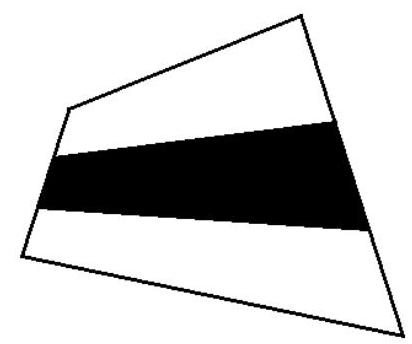
\includegraphics[max width=\textwidth, center]{2024_11_21_90af61d06b3c3adeff73g-1}


\end{document}